%\chapter{Anhänge}
\chapter{Detailed Derivations and Results} \label{c:A}

\section{Differentiable GP Kernels} \label{sec:A.1}

A key property of many kernel functions used in Gaussian process regression is smoothness, which is directly related to differentiability. In this section, we examine the differentiability properties of the widely-used squared exponential (SE) or a radial basis function (RBF) kernel, which is infinitely differentiable and thus yields a Gaussian process prior over smooth functions \cite{RasmussenW06, Solak2002}.

Before examining a squared exponential kernel and its derivative, we initially define the squared exponential kernel as
\begin{equation} \label{equ:A.1}
    k(\mathbf{x},\;\mathbf{x}^{*}) = \sigma_{o} \exp\left(-\frac{1}{2\ell^2} \|\mathbf{x} - \mathbf{x}^{*}\|^2\right),
\end{equation}
where $\sigma_{o}$ is the  , $\ell$ is the length scale, and $\|\cdot\|$ denotes the Euclidean norm. The kernel depends on the squared distance between input vectors, making it isotropic and stationary.

\subsection{Arbitrary Order Derivatives} \label{sec:A.1.1}

Since the SE kernel is infinitely differentiable with respect to both arguments $\mathbf{x}$ and $\mathbf{x}^{*}$,  this property allows us to compute analytic gradients and higher-order derivatives, which are crucial for modelling derivatives of functions (e.g., force fields, gradient, and higher-order derivative observations) or constructing physically informed models.

I begin with deriving from the first- up to sixth-order derivatives which are essential for the predictive means and varainces of Gaussian process forces constant, i.e., defined in Equation \eqref{equ:3.7}, \eqref{equ:3.9}, and \eqref{equ:3.26}.

The first order derivative of the kernel with respect to $\mathbf{x}$ can be derived
To compute the first-order partial derivative of $k(\mathbf{x},\;\mathbf{x}^*)$ with respect to component $x_i$ of $\mathbf{x}$, we first define $\mathbf{r}=\mathbf{x} - \mathbf{x}^{*}$ and its Euclidean distance
\[
\mathbf{r}^2(\mathbf{x},\;\mathbf{x}^{*}) = \|\mathbf{x} - \mathbf{x}^{*}\|^2 = \sum_{j=1}^d (x_j - x_j^*)^2,
\]
where $\mathbf{x},\;\mathbf{x}^{*}\in\mathbb{R}^{d}$. The kernel then becomes:
\[
k(\mathbf{x},\;\mathbf{x}^*) = \sigma_{o} \exp\left( -\frac{1}{2\ell^2} \mathbf{r}^2 \right),
\]
which is analougous to \eqref{equ:3.1}.
Now the gradient of the kernel can be evaluated using the chain rule:
\begin{align}
\frac{\partial k}{\partial x_i} 
&= \frac{\mathrm{d}k}{\mathrm{d}\mathbf{r}^2} \cdot \frac{\partial r^2}{\partial x_i} \notag \\
&= \left( -\frac{1}{2\ell^2} k(\mathbf{x},\;\mathbf{x}^*) \right) \cdot 2(x_i - x_i^*) \notag \\
&= -\frac{1}{\ell^2} k(\mathbf{x},\;\mathbf{x}^*)\,(x_i - x_i^*).\label{equ:A.2}
\end{align}
Thus, we can represent it in the form of the $d$-dimensional vector given by
\begin{equation} \label{equ:A.3}
\boxed{
    \nabla_{\mathbf{x}} k(\mathbf{x},\;\mathbf{x}^*) =
    -\frac{1}{\ell^2} k(\mathbf{x},\;\mathbf{x}^*)
    \cdot\mathbf{r}.
    }
\end{equation}
Likewise, the gradient with respect to $\mathbf{x}^{*}$ is expressed as
\begin{equation} \label{equ:A.4}
\boxed{
    \nabla_{\mathbf{x}^{*}} k(\mathbf{x},\;\mathbf{x}^*) = 
    \frac{1}{\ell^2} k(\mathbf{x},\;\mathbf{x}^*)
    \cdot\mathbf{r},
    }
\end{equation}
which is the antisymmetric form of Eq. \eqref{equ:A.3}.

We can now compute the second-order derivative of the squared exponential kernel with respect to the $j$-th component of $\mathbf{x}$:
\[
\frac{\partial^2 k}{\partial x_i \partial x_j} = \frac{\partial}{\partial x_j} \left( \frac{\partial k}{\partial x_i} \right).
\]
This calculation is divided into two cases: $i=j$ and $i\neq j$.
Using the first derivative solution in \eqref{equ:A.3}, we compute the second-order partial derivative of the kernel with respect to $x_j = x_i$ for the first case, resulting in
\begin{align} \label{equ:A.5}
\frac{\partial^2 k(\mathbf{x},\;\mathbf{x}^*)}{\partial x_i^2}
&= \frac{\partial}{\partial x_i} \left[ -\frac{1}{\ell^2} (x_i - x_i^*) \, k(\mathbf{x},\;\mathbf{x}^*) \right] \notag \\
&= -\frac{1}{\ell^2} \left[ \frac{\partial}{\partial x_i} (x_i - x_i^*) \cdot k(\mathbf{x},\;\mathbf{x}^*) + (x_i - x_i^*) \cdot \frac{\partial k(\mathbf{x},\;\mathbf{x}^*)}{\partial x_i} \right] \notag \\
&= -\frac{1}{\ell^2} \left[ k(\mathbf{x},\;\mathbf{x}^*) - \frac{1}{\ell^2} (x_i - x_i^*)^2 \, k(\mathbf{x},\;\mathbf{x}^*) \right] \notag \\
&= \left( \frac{1}{\ell^4}(x_i - x_i^*)^2 - \frac{1}{\ell^2} \right) k(\mathbf{x},\;\mathbf{x}^*).
\end{align}
For the second case, cross-differentiating with respect to $x_j \neq x_i$ yields
\begin{align} \label{equ:A.6}
\frac{\partial^2 k(\mathbf{x},\;\mathbf{x}^*)}{\partial x_i \partial x_j}
&= \frac{\partial}{\partial x_j} \left( -\frac{1}{\ell^2} (x_i - x_i^*) \, k(\mathbf{x},\;\mathbf{x}^*) \right) \notag \\
&= -\frac{1}{\ell^2} (x_i - x_i^*) \cdot \frac{\partial k(\mathbf{x},\;\mathbf{x}^*)}{\partial x_j} \notag \\
&= -\frac{1}{\ell^2} (x_i - x_i^*) \cdot \left( -\frac{1}{\ell^2} (x_j - x_j^*) \, k(\mathbf{x},\;\mathbf{x}^*) \right) \notag \\
&= \frac{1}{\ell^4} (x_i - x_i^*)(x_j - x_j^*) \, k(\mathbf{x},\;\mathbf{x}^*).
\end{align}
Combining the solutions in \eqref{equ:A.5} and \eqref{equ:A.6}, the second derivative is expressed as a rank-2 tensor or a $d\times d$ matrix
\begin{equation}  \label{equ:A.7}
\boxed{
(\nabla_{\mathbf{x}})^{2} k(\mathbf{x},\;\mathbf{x}^*) = 
\left( \frac{1}{\ell^4} \mathbf{r} \otimes \mathbf{r}
- \frac{1}{\ell^2} \mathbb{1} \right) k(\mathbf{x},\;\mathbf{x}^*),
}
\end{equation}
where $\mathbb{1}$ is a $(d\times d)$ identity matrix.
\begin{figure*}[t]\centering
  \centering
  
\includegraphics[width=0.5\linewidth,height=\textheight,keepaspectratio]{Figure/Appendix/DeriGP/012.jpg}
    \caption{
        \label{fig:A.1}
        Construction of the derivative kernel (covariance) matrix used in our GP model.
        Each block $(m,n)$ represents the $(m+n)$th-order kernel derivative $(\nabla_{\mathbf{x}})^{m} (\nabla_{\mathbf{x}^*})^{m} k(\mathbf{x}, \mathbf{x}^*)$ which behaves as a rank-$(m+n)$ tensor. For all $\mathbf{x},\;\mathbf{x}^*\in\mathbb{R}^{d}$,this tensor is reshaped into a $(d^{m}\times d^{n})$-matrix to construct the whole covariance matrix. 
    }
\end{figure*}
Similarly, the mixed partial derivative of the squared exponential kernel with respect to $\mathbf{x}$ and $\mathbf{x}^*$ is expressed as
\begin{equation} \label{equ:A.8}
\boxed{
\nabla_{\mathbf{x}} \nabla_{\mathbf{x}^*} k(\mathbf{x},\;\mathbf{x}^*) = 
\left( -\frac{1}{\ell^4} \mathbf{r} \otimes \mathbf{r} 
+ \frac{1}{\ell^2} \mathbb{1} \right) k(\mathbf{x},\;\mathbf{x}^*),
}
\end{equation}
and the second derivative with respect to $\mathbf{x}^*$ and $\mathbf{x}^*$ is given by
\begin{equation} \label{equ:A.9}
\boxed{
(\nabla_{\mathbf{x}^*})^{2} k(\mathbf{x},\;\mathbf{x}^*) = 
\left( \frac{1}{\ell^4} \mathbf{r} \otimes \mathbf{r}
- \frac{1}{\ell^2} \mathbb{1} \right) k(\mathbf{x},\;\mathbf{x}^*).
}
\end{equation}
By examining these three second-order derivative solutions, we can form the symmetric relation among them as follows
\begin{equation} \label{equ:A.10}
\boxed{
(\nabla_{\mathbf{x}})^{2} k(\mathbf{x},\;\mathbf{x}^*)=
-\nabla_{\mathbf{x}} \nabla_{\mathbf{x}^*} k(\mathbf{x},\;\mathbf{x}^*)=
(\nabla_{\mathbf{x}^*})^{2} k(\mathbf{x},\;\mathbf{x}^*)  
.
}
\end{equation}

The SE kernel, along with the solutions of its first- and second-order derivatives, can be used to construct the covariance matrix depicted in Figure \ref{fig:A.1}.
This matrix construction provides the systematic classification of the $(m+n)$th-order kernel derivative $(\nabla_{\mathbf{x}})^{m} (\nabla_{\mathbf{x}^*})^{n} k(\mathbf{x}, \mathbf{x}^*)$, where the oreder $m$ and $n$ increase along the diagonal direction. Each $(\nabla_{\mathbf{x}})^{m} (\nabla_{\mathbf{x}^*})^{n} k(\mathbf{x}, \mathbf{x}^*)$ is denoted by the block $(m,n)$.
For example, the SE kernal is the block $(0,0)$ whereas the block $(2,0)$ represents the second-order derivative given in \eqref{equ:A.7}.

Moreover, this matrix assists us in identifying the (anti)symmetry of the kernel derivative in the same order.
Specifically, block matrices of identical colour that align along the same antidiagonal exhibit correlation due to their (anti)symmetric property.
The blocks $(2,0)$, $(1,1)$, and $(0,2)$ exemplify the (anti)symmetric property defined in \eqref{equ:A.10}.
This matrix construction will become more evident after completing all the blocks.

Let us consider the third-order derivative of the kernel.
Correlating the symmetric property of the relevant blocks--specifically, $(3,0)$, $(2,1)$, $(1,2)$, and $(0,3)$--allow us to formulate
\begin{equation} \label{equ:A.11}
\boxed{
(\nabla_{\mathbf{x}})^{3} k=
-(\nabla_{\mathbf{x}})^{2} \nabla_{\mathbf{x}^*} k=
\nabla_{\mathbf{x}} (\nabla_{\mathbf{x}^*})^{2} k=
-(\nabla_{\mathbf{x}^*})^{3} k 
.
}
\end{equation}
Accordingly, the construction of all third-order derivative blocks requires the calculation of only a single representative term, from which the remaining components follow by symmetry.
We then solve the solution of the third-order derivative with respect to components $x_i$, $x_j$, and $x_k$ of $\mathbf{x}$:
\[
\frac{\partial^3 k}{\partial x_i \partial x_j \partial x_k}.
\]
We begin with applying the product rule to differentiate the Hessian component of Equation \eqref{equ:A.7}, yielding
\[
\frac{\partial^3 k}{\partial x_i \partial x_j \partial x_k}
= \frac{\partial}{\partial x_k} \left( \frac{\partial^2 k}{\partial x_i \partial x_j} \right)
= \frac{\partial}{\partial x_k} \left[ \left( \frac{1}{\ell^4} r_i r_j - \frac{1}{\ell^2} \delta_{ij} \right) k \right].
\]
The product rule is, now, employed to obtain
\begin{align} \label{equ:A.12}
\frac{\partial^3 k}{\partial x_i \partial x_j \partial x_k}
&= \left( \frac{1}{\ell^4} \delta_{ik} r_j + \frac{1}{\ell^4} r_i \delta_{jk} \right) k
+ \left( \frac{1}{\ell^4} r_i r_j - \frac{1}{\ell^2} \delta_{ij} \right) \frac{\partial k}{\partial x_k}.
\end{align}
We substitute the gradient solution given in \eqref{equ:A.2}, resulting in 
\begin{align} \label{equ:A.13}
\frac{\partial^3 k}{\partial x_i \partial x_j \partial x_k}
&= \left( \frac{1}{\ell^4} \delta_{ik} r_j + \frac{1}{\ell^4} r_i \delta_{jk} \right) k
- \left( \frac{1}{\ell^4} r_i r_j - \frac{1}{\ell^2} \delta_{ij} \right) \frac{1}{\ell^2} r_k \, k \notag \\
&= \left[ \frac{1}{\ell^4} (\delta_{ik} r_j + \delta_{jk} r_i) 
- \frac{1}{\ell^6} r_i r_j r_k + \frac{1}{\ell^4} \delta_{ij} r_k \right] k.
\end{align}
Therefore, the final expression is given by
\begin{equation} \label{equ:A.14}
\boxed{
\frac{\partial^3 k}{\partial x_i \partial x_j \partial x_k}
=
\left[
    -\frac{1}{\ell^6} r_i r_j r_k
    + \frac{1}{\ell^4} \left( \delta_{ij} r_k + \delta_{ik} r_j + \delta_{jk} r_i \right)
\right]
k(\mathbf{x},\;\mathbf{x}^*).
}
\end{equation}

\begin{figure*}[t]\centering
  \centering
  
\includegraphics[width=0.5\linewidth,height=\textheight,keepaspectratio]{Figure/Appendix/DeriGP/0_6.jpg}
    \caption{
        \label{fig:A.2}
        Complete construction of the derivative kernel matrix used in our GP model. 
    }
\end{figure*}
We now proceed to populate the third-order derivative blocks \((3,0)\), \((2,1)\), \((1,2)\), and \((0,3)\), as illustrated in Figure~\ref{fig:A.2}. To evaluate the remaining higher-order derivative blocks—namely the fourth-order \((3,1)\), \((2,2)\), \((1,3)\); the fifth-order \((3,2)\), \((2,3)\); and the sixth-order \((3,3)\)—we similarly employ the (anti)symmetry relations between the mixed Wirtinger derivatives, as follows:
\begin{itemize}
    \item \textbf{Fourth-order} (involving \((\nabla_{\mathbf{x}})^4 k\)):
    \[
    \boxed{
    (\nabla_{\mathbf{x}})^3 \nabla_{\mathbf{x}^*} k =
    -(\nabla_{\mathbf{x}})^2 (\nabla_{\mathbf{x}^*})^2 k =
    \nabla_{\mathbf{x}} (\nabla_{\mathbf{x}^*})^3 k :=
    -(\nabla_{\mathbf{x}})^4 k.
    }
    \]
    
    \item \textbf{Fifth-order} (involving \((\nabla_{\mathbf{x}})^5 k\)):
    \[
    \boxed{
    (\nabla_{\mathbf{x}})^3 (\nabla_{\mathbf{x}^*})^2 k =
    -(\nabla_{\mathbf{x}})^2 (\nabla_{\mathbf{x}^*})^3 k =
    (\nabla_{\mathbf{x}})^5 k.
    }
    \]
    
    \item \textbf{Sixth-order} (involving \((\nabla_{\mathbf{x}})^6 k\)):
    \[
    \boxed{
    (\nabla_{\mathbf{x}})^3 (\nabla_{\mathbf{x}^*})^3 k :=
    -(\nabla_{\mathbf{x}})^6 k.
    }
    \]
\end{itemize}
To evaluate the required derivatives—\((\nabla_{\mathbf{x}})^4 k\), \((\nabla_{\mathbf{x}})^5 k\), and \((\nabla_{\mathbf{x}})^6 k\)—one must additionally apply both the product rule and the chain rule, in a manner analogous to the third-order case discussed in Equations~\eqref{equ:A.12}–\eqref{equ:A.14}.

Rather than presenting full derivations, I will provide the solutions associated to those three cases.
Beginning with the fourth-order, its components are given by
\begin{equation} \label{equ:A.15}
\begin{aligned}
\frac{\partial^4 k}{\partial x_i \partial x_j \partial x_k \partial x_a}
= \Big[ &
\frac{1}{\ell^8} r_i r_j r_k r_a \\
&- \frac{1}{\ell^6} \big(
    \delta_{ij} r_k r_a + \delta_{ik} r_j r_a + \delta_{ia} r_j r_k \\
    &+ \delta_{jk} r_i r_a + \delta_{ja} r_i r_k + \delta_{ka} r_i r_j
\big) \\
&+ \frac{1}{\ell^4} \big(
    \delta_{ij} \delta_{ka} + \delta_{ik} \delta_{ja} + \delta_{ia} \delta_{jk}
\big)
\Big] \, k(\mathbf{x},\;\mathbf{x}^*).
\end{aligned}
\end{equation}
We can rewrite the expression in terms of symmetrised permutation notation, yielding
\begin{equation} \label{equ:A.16}
\boxed{
\frac{\partial^4 k}{\partial x_i \partial x_j \partial x_k \partial x_a}
=
\left[
\frac{1}{\ell^8} r_i r_j r_k r_a
- \frac{6}{\ell^6} \, \delta_{(ij} r_k r_{a)}
+ \frac{3}{\ell^4} \, \delta_{(ij} \delta_{ka)}
\right] k(\mathbf{x},\;\mathbf{x}^*)
}
\end{equation}
where the parentheses $(\cdot)$ denote symmetrisation over the enclosed indices.

Finally, the fifth- and the sixth-order derivatives can be expressed in the symmetrised permutation noatation as 
\begin{equation} \label{equ:A.17}
\boxed{
\begin{aligned}
\frac{\partial^5 k}{\partial x_i \partial x_j \partial x_k \partial x_a \partial x_b}
= \Big[ &
- \frac{1}{\ell^{10}} r_i r_j r_k r_a r_b \\
&+ \frac{10}{\ell^8} \, \delta_{(ij} r_k r_a r_{b)} \\
&- \frac{15}{\ell^6} \, \delta_{(ij} \delta_{ka} r_{b)}
\Bigg] k(\mathbf{x},\;\mathbf{x}^*),
\end{aligned}
}
\end{equation}
and
\begin{equation} 
\boxed{
\begin{aligned}
\frac{\partial^6 k}{\partial x_i \partial x_j \partial x_k \partial x_a \partial x_b \partial x_c}
= \Bigg[ &
\frac{1}{\ell^{12}} \, r_i r_j r_k r_a r_b r_c \\
&- \frac{15}{\ell^{10}} \, \delta_{(ij} r_k r_a r_b r_{c)} \\
&+ \frac{45}{\ell^8} \, \delta_{(ij} \delta_{ka} r_b r_{c)} \\
&- \frac{15}{\ell^6} \, \delta_{(ij} \delta_{ka} \delta_{bc)} 
\Bigg] k(\mathbf{x},\;\mathbf{x}^*),
\end{aligned}
}
\end{equation}
respectively.

In the following section, I will present a sophisticated framework for developing the differentiable Gaussian Process model to accommodate complex representations, such as phonon descriptors.

%\subsection{Extension to Non-Euclidean Metrics}

%Although Equation~\eqref{eq:se-kernel} assumes a Euclidean metric, it is straightforward to generalize the kernel to use a Mahalanobis distance defined by a positive definite matrix $M$:
%\begin{equation}
%    d_M^2(\mathbf{x}, \mathbf{x}^{*}) = (\mathbf{x} - \mathbf{x}^{*})^\top M (\mathbf{x} - \mathbf{x}^{*}).
%\end{equation}
%This modification allows for anisotropic modeling where different directions in input space have distinct length scales.
\newpage
\subsection{Complex Gaussian Process} \label{sec:A.1.2}
In this section, we investigate the kernel function, which supports complex vectors, and its derivative with respect to these vectors.
Deriving these derivatives allows us to build the differentiable GP model supporting phonon descriptors evaluated at arbitary wavevectors $\mathbf{q}$. 
These phonon descriptors are currently not compatible with our GP model, while the phonon descriptor evaluated at $\Gamma$-point $(\mathbf{q}=0)$ is only the case that can be applied to our model, as discussed in section \ref{sec:3.2}.

We begin with consider a squared exponential kernel defined on complex vectors \(\mathbf{z},\;\mathbf{z}^* \in \mathbb{C}^d\), where
\[
\mathbf{z} = \mathbf{a} + i \mathbf{b}, \quad \mathbf{z}^* = \mathbf{a}^* + i \mathbf{b}^*, \quad \text{with } \mathbf{a}, \mathbf{b} \in \mathbb{R}^d.
\]

The squared exponential kernel can be rewritten as
\begin{equation} \label{equ:A.19}
    k(\mathbf{z},\;\mathbf{z}^*) = \sigma_{o} \exp\left( -\frac{1}{2\ell^2} \|\mathbf{z} - \mathbf{z}^*\|^2 \right),
\end{equation}
where
\[
\|\mathbf{z} - \mathbf{z}^*\|^2 := (\mathbf{z} - \mathbf{z}^*)^\dagger (\mathbf{z} - \mathbf{z}^*) = \sum_{j=1}^d |z_j - z_j^*|^2,
\]
ensuring that \(k\) is real-valued and positive definite.

To diffentiate the kernel requires to define the \textit{Wirtinger} derivatives with respect to the complex coordinates:
\[
\frac{\partial}{\partial z_i} := \frac{1}{2} \left( \frac{\partial}{\partial a_i} - i \frac{\partial}{\partial b_i} \right), \qquad
\frac{\partial}{\partial \overline{z}_i} := \frac{1}{2} \left( \frac{\partial}{\partial a_i} + i \frac{\partial}{\partial b_i} \right).
\]

The first-order derivatives of the kernel are given by:
\begin{equation} \label{equ:A.20}
\boxed{
\begin{aligned}
\frac{\partial k(\mathbf{z},\;\mathbf{z}^*)}{\partial z_i} &= -\frac{1}{\ell^2} (z_i - z_i^*) \, k(\mathbf{z},\;\mathbf{z}^*),  
\end{aligned}
}
\end{equation}
\begin{equation} \label{equ:A.21}
\boxed{
\begin{aligned}
\frac{\partial k(\mathbf{z},\;\mathbf{z}^*)}{\partial \overline{z}_i} &= -\frac{1}{\ell^2} (\overline{z}_i - \overline{z}_i^*) \, k(\mathbf{z},\;\mathbf{z}^*). 
\end{aligned}
}
\end{equation}

These expressions respect \textit{Holomorphic}\footnote{A function is considered holomorphic if it is complex differentiable in an open neighbourhood, a characteristic that entails infinite differentiability and analyticity as a result of fulfilling the Cauchy-Riemann equations.  This concept is fundamental to complex analysis and is essential for deriving derivatives through Wirtinger calculus \cite{stein2003}.} structure when treating \(\mathbf{z}\) and \(\mathbf{z}^*\) as independent formal variables. Higher-order Wirtinger derivatives follow similarly and preserve symmetry under complex conjugation.

We can also take the \textit{Wirtinger} derivative of the kernel with respect to $\mathbf{z}^*$ and $\overline{\mathbf{z}}^*$, resulting in the similar results as Equation \eqref{equ:A.4}.

Computing the second-order derivatives can be divided into two cases.
One is the pure (holomophic) second derivative with respect to \(\mathbf{z}\) and \(\mathbf{z}\):
\begin{align} \label{equ:A.22}
\frac{\partial^2 k}{\partial z_i \partial z_j} 
&= \frac{\partial}{\partial z_j} \left[ -\frac{1}{\ell^2} (z_i - z_i^*)\, k \right] \notag \\
&= -\frac{1}{\ell^2} \delta_{ij} \, k + \frac{1}{\ell^4} (z_i - z_i^*)(z_j - z_j^*)\, k,
\end{align}
which can be expressed as
\begin{equation} \label{equ:A.23}
\boxed{
\frac{\partial^2 k}{\partial z_i \partial z_j} 
= \left( \frac{1}{\ell^4} (z_i - z_i^*)(z_j - z_j^*) - \frac{1}{\ell^2} \delta_{ij} \right) k.
}
\end{equation}
This result is defined as the component $i,\;j$ of the rank-2 tensor \(\nabla^{2}_{\mathbf{z}\mathbf{z}}k\).
Meanwhile, the mixed derivative with respect to \(\mathbf{z}\) and \(\overline{\mathbf{z}}\) can be solved as follows 
\begin{align} \label{equ:A.24}
\frac{\partial^2 k}{\partial z_i \partial \overline{z}_j}
&= \frac{\partial}{\partial \overline{z}_j} \left[ -\frac{1}{\ell^2} (z_i - z_i^*)\, k \right] \notag \\
&= -\frac{1}{\ell^2} (z_i - z_i^*) \cdot \frac{\partial k}{\partial \overline{z}_j} \notag \\
&= -\frac{1}{\ell^2} (z_i - z_i^*) \cdot \left( -\frac{1}{\ell^2} (\overline{z}_j - \overline{z}_j^*)\, k \right) \notag \\
&= \frac{1}{\ell^4} (z_i - z_i^*)(\overline{z}_j - \overline{z}_j^*)\, k,
\end{align}
yielding
\begin{equation} \label{equ:A.25}
\boxed{
\frac{\partial^2 k}{\partial z_i \partial \overline{z}_j} 
= \frac{1}{\ell^4} (z_i - z_i^*)(\overline{z}_j - \overline{z}_j^*)\, k
}
\end{equation}
as the component $i,\;j$ of the rank-2 tensor \(\nabla^{2}_{\mathbf{z}\overline{\mathbf{z}}}k\).

%We can see that these two solutions are analogous Equation \eqref{equ:A.5} and \eqref{equ:A.6}, which they can be rewritten with $\delta_{z\overline{z}}$ on the second as

To obtain the remaining second order derivatives, i.e. \(\nabla^{2}_{\overline{\mathbf{z}}\overline{\mathbf{z}}}k\) and \(\nabla^{2}_{\overline{\mathbf{z}}\mathbf{z}}k\), requires to use the conjugation of derivative identity defined as
\begin{align} \label{equ:A.26} 
\overline{ \left( \frac{\partial f}{\partial z_i} \right) } &= \frac{\partial f}{\partial \overline{z}_i}, 
\end{align}
for \( f: \mathbb{C}^d \rightarrow \mathbb{R} \) be a real-valued, smooth function of complex variables.
They can, therefore, evaluated through the relations
\begin{align} 
 \nabla^{2}_{\overline{\mathbf{z}}\overline{\mathbf{z}}}k &= \overline{\nabla^{2}_{\mathbf{z}\mathbf{z}}k}, \label{equ:A.27}\\ 
 \nabla^{2}_{\overline{\mathbf{z}}\mathbf{z}}k &= \overline{\nabla^{2}_{\mathbf{z}\overline{\mathbf{z}}}k}. \label{equ:A.28}
\end{align}

Combining Equation \eqref{equ:A.23}, \eqref{equ:A.25}, \eqref{equ:A.27}, and \eqref{equ:A.28} allow us to form the full description of the second order derivative with respect to \(\mathbf{z}\) and \(\overline{\mathbf{z}}\), defined as a $(2d\times 2d)$-matrix:
\begin{equation} \label{equ:A.29}
    \tilde{D}^{2}_{\mathbf{z}\mathbf{z}}k=
    \begin{bmatrix}
       \nabla^{2}_{\mathbf{z}\mathbf{z}}k & \nabla^{2}_{\mathbf{z}\overline{\mathbf{z}}}k
        \\
        \nabla^{2}_{\overline{\mathbf{z}}\mathbf{z}}k & \nabla^{2}_{\overline{\mathbf{z}}\overline{\mathbf{z}}}k
    \end{bmatrix}.
\end{equation}
The diagonal block matrices $\nabla^{2}_{\mathbf{z}\mathbf{z}}k$ and $\nabla^{2}_{\overline{\mathbf{z}}\overline{\mathbf{z}}}k$ denote the standard second-order holomorphic derivative and its anti-holomorphic counterpart, respectively. 
The existence of both real and imaginary values in these two blocks causes themselves generally unphysical.
Meanwhile, the off-diagonal blocks $\nabla^{2}_{\mathbf{z}\overline{\mathbf{z}}}k$ and $ \nabla^{2}_{\overline{\mathbf{z}}\mathbf{z}}k$ exhibit physical properties, as they are Hermitian conjugates of each other.

To construct the differential GP model for predicting harmonic force constants, analogous to \eqref{equ:3.7}, also requires to evaluate the third-order derivatives with respect to those complex vectors.

Regarding the symmetric conjugation property, only three cases are adequate to populate all solutions for the third order derivative.

We begin with defining \( r_i := z_i - z_i^* \), and \( \bar{r}_i := \bar{z}_i - \bar{z}_i^* \). The third-order Wirtinger derivatives of the complex squared exponential kernel
are given by
\paragraph{(i) Holomorphic third derivative:}
\begin{equation} \label{equ:A.30}
\boxed{
\frac{\partial^3 k}{\partial z_i \partial z_j \partial z_k}
= \left( 
  -\frac{1}{\ell^6} r_i r_j r_k 
  + \frac{3}{\ell^4} \delta_{(ij} r_{k)} 
\right) k,
}
\end{equation}

\paragraph{(ii) Mixed two holomorphic, one antiholomorphic:}
\begin{equation} \label{equ:A.31}
\boxed{
\frac{\partial^3 k}{\partial z_i \partial z_j \partial \overline{z}_k}
= \left( 
  -\frac{1}{\ell^6} r_i r_j \bar{r}_k 
  + \frac{1}{\ell^4} \delta_{ij} \bar{r}_k 
\right) k,
}
\end{equation}

\paragraph{(iii) Mixed one holomorphic, two antiholomorphic:}
\begin{equation} \label{equ:A.32}
\boxed{
\frac{\partial^3 k}{\partial z_i \partial \overline{z}_j \partial \overline{z}_k}
= \left( 
  -\frac{1}{\ell^6} r_i \bar{r}_j \bar{r}_k 
  + \frac{1}{\ell^4} \delta_{jk} r_i 
\right) k.
}
\end{equation}
These are the components $i,\;j,\;k$ of $\nabla^{3}_{\mathbf{z}\mathbf{z}\mathbf{z}}k$, $\nabla^{3}_{\mathbf{z}\mathbf{z}\overline{\mathbf{z}}}k$  and $\nabla^{3}_{\mathbf{z}\overline{\mathbf{z}}\overline{\mathbf{z}}}k$, respectively.
We can employ the conjugation of derivative identity and the permutation symmetry to achieve the following relation
\begin{align} 
 \overline{\nabla^{3}_{\mathbf{z}\mathbf{z}\mathbf{z}}k} &= \nabla^{3}_{\overline{\mathbf{z}}\overline{\mathbf{z}}\overline{\mathbf{z}}}k, \label{equ:A.33}\\ 
 \nabla^{3}_{\mathbf{z}\mathbf{z}\overline{\mathbf{z}}}k = \nabla&^{3}_{\mathbf{z}\overline{\mathbf{z}}\mathbf{z}}k = 
 \nabla ^{3}_{\overline{\mathbf{z}}\mathbf{z}\mathbf{z}}k, \label{equ:A.34}\\
 \nabla^{3}_{\mathbf{z}\overline{\mathbf{z}}\overline{\mathbf{z}}}k =
 \nabla&^{3}_{\overline{\mathbf{z}}\overline{\mathbf{z}}\mathbf{z}}k = 
 \nabla ^{3}_{\overline{\mathbf{z}}\mathbf{z}\overline{\mathbf{z}}}k. \label{equ:A.35}
\end{align}

\begin{figure*}[t]
\centering
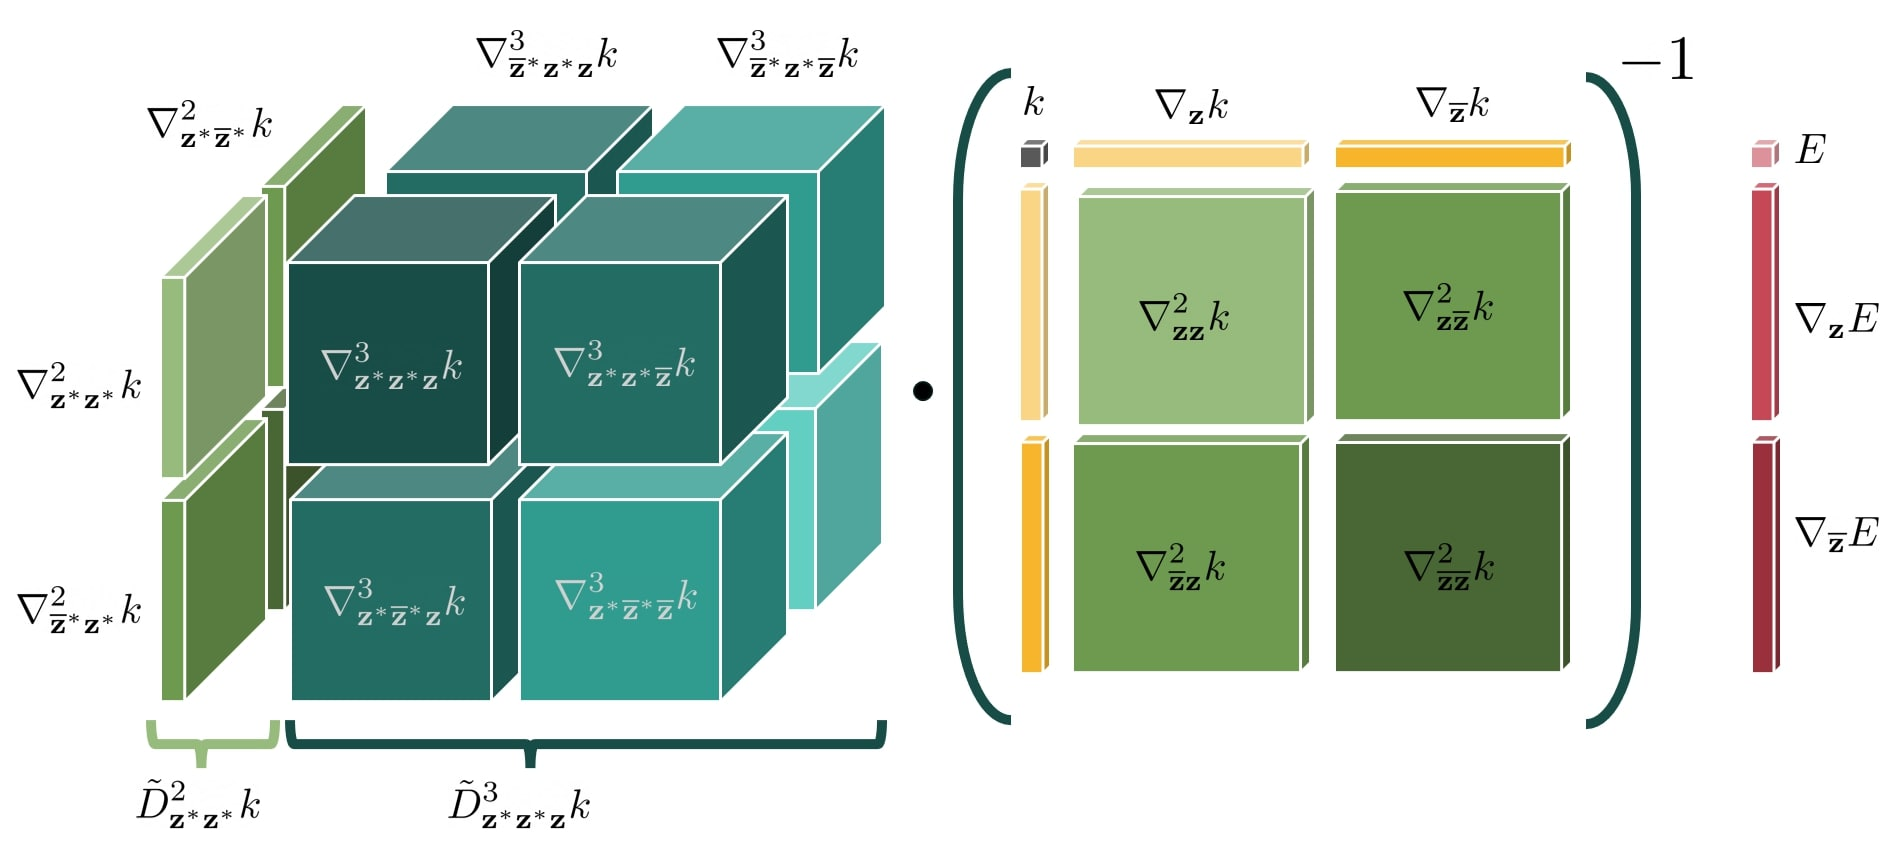
\includegraphics[width=1.0\textwidth]{Figure/Appendix/DeriGP/complex_deri.jpg}
\caption{\label{fig:A.3} Figure illustrates the tensor contraction in Equation~\eqref{equ:A.37}, where the derivative GP model is trained on a single data point at descriptor $\mathbf{z}$. This serve as an extension to the tensor contraction shown in Fig. \ref{fig:3.1} and \ref{fig:3.7}.}
\end{figure*}
We can now construct the full third order derivative with respect to \(\mathbf{z}\) and \(\overline{\mathbf{z}}\), defined as a rank-3 tensor with size $2d\times 2d \times 2d$:
\begin{equation} \label{equ:A.36}
    \tilde{D}^{3}_{\mathbf{z}\mathbf{z}\mathbf{z}}k=\left\{
    \begin{bmatrix}
    \nabla^{3}_{\mathbf{z}\mathbf{z}\mathbf{z}}k & \nabla^{3}_{\mathbf{z}\mathbf{z}\overline{\mathbf{z}}}k \\
\nabla^{3}_{\mathbf{z}\overline{\mathbf{z}}\mathbf{z}}k & \nabla^{3}_{\mathbf{z}\overline{\mathbf{z}}\overline{\mathbf{z}}}k
\end{bmatrix},
\begin{bmatrix}
\nabla^{3}_{\overline{\mathbf{z}}\mathbf{z}\mathbf{z}}k & 
\nabla ^{3}_{\overline{\mathbf{z}}\mathbf{z}\overline{\mathbf{z}}}k \\
\nabla^{3}_{\overline{\mathbf{z}}\overline{\mathbf{z}}\mathbf{z}}k & 
\nabla^{3}_{\overline{\mathbf{z}}\overline{\mathbf{z}}\overline{\mathbf{z}}}k
\end{bmatrix}
    \right\}.
\end{equation}
Therefore, our diffrential GP model, for predicting the second oreder force constants in both the Cartesian \eqref{equ:3.7} and the phonon basis \eqref{equ:3.19}, can be rewritten to support the complex vectors as
\begin{tcolorbox}[
    ams equation,
    title=Wirtinger  GPFC2 ,
    %colback=blue!5,
    colframe=bEpic,
    %colframe=blue!75!black,
    coltitle=white,
    %fontupper=\color{blue}  % << changes font color inside the box
]
\label{equ:A.37}
\begin{split}
    \Phi^{(2)}(\mathbf{z}^{*}) = 
    \begin{bmatrix}
          \tilde{D}^{2}_{\mathbf{z}^{*}\mathbf{z}^{*}}k\\
          \tilde{D}^{3}_{\mathbf{z}^{*}\mathbf{z}^{*}\mathbf{z}}k
    \end{bmatrix}_{\textbf{z},\;\textbf{z}^{*}}^{\text{T}}
        \cdot \begin{bmatrix}
              k & (\tilde{D}_{\mathbf{z}}k)^{\text{T}}\\
              \tilde{D}_{\mathbf{z}}k & \tilde{D}^{2}_{\mathbf{z}^{*}\mathbf{z}^{*}}k \\
        \end{bmatrix}^{-1}_{\mathbf{z},\: \mathbf{z}}
        \cdot
        \begin{bmatrix}
              E \\
              \nabla_{\mathbf{z}} E\\
              \nabla_{\overline{\mathbf{z}}} E\\
        \end{bmatrix}_{\mathbf{z}},
\end{split}
\end{tcolorbox}
where
\[ \tilde{D}_{\mathbf{z}}k=\begin{bmatrix}
              \nabla_{\mathbf{z}} k&
              \nabla_{\overline{\mathbf{z}}} k
        \end{bmatrix}.\]
Here, $\nabla_{\mathbf{z}} E$ and $\nabla_{\overline{\mathbf{z}}} E$ correspond to the forces defined on complex vector $\mathbf{z}$. They can, particularly, be obtained using the transformation to transform Cartesian forces into the phonon coordinate at arbitrary $\mathbf{q}$-wavevector.

Subsequent to the prediction, we will acquire the \(2d\times2d\) complex GPFC2 \[ \Phi^{(2)}(\mathbf{z}^{*}):=\Phi^{(2)}(\mathbf{z}^{*},\;\overline{\mathbf{z}}^{*}).\]
This corresponds to the \(12\times12\) dynamical matrix for a \(2\times2\times2\) supercell of a diatomic crystal structure, such as d-\textbf{Si}, \textbf{PbTe}, and \textbf{NaCl}, which is inconsistent.
However, we can use the fact that the \(6\times6\) off-diagonal block matrices are non-holomophic (or physical). 
This is due to the fact that these off-diagonal block matrices depend on both \(\mathbf{z}^{*}\) and \(\overline{\mathbf{z}}^{*}\), while the diagonal block matrices depend only on \(\mathbf{z}^{*}\) (or \(\overline{\mathbf{z}}^{*}\)).
This \(\mathbf{z}^{*}\)- (or \(\overline{\mathbf{z}}^{*}\)-)dependence leads to (anti)holomorphism, preventing the definition of the Hermitian property.
Therefore, the real (physical) dynamical matrix should be equivalent one of the \(6\times6\) off-diagonal block matrices, with the other block being its Hermitian matrix.

In the case of the cubic anharmonic force constants, this Wirtinger derivative GP model requires the fourth-order derivative for the extension to support phonon-based GPFC3 prediction.  

%Therefore, a dynamical matrices and FC3 in phonon basis can only be evaluated at $\Gamma$ point, where the phonon descriptor are real.

%To overcome this limitation, we begin with modifying the RBF kernel in Equation \eqref{equ:3.1} to support the descriptor $\mathbf{z}$ in the complex vector space, i.e., 
%\[\mathbf{z}=\mathbf{a}+i\mathbf{b},\]
%where $\mathbf{a}$ and $\mathbf{b}$ are in the real vector space. By assuming the real kernel function, the RBF kernel can be redefined as
%\begin{equation} \label{equ:3.20}
   %     \begin{split}
   %         k(\mathbf{z},\;\mathbf{z}^{*})= \sigma_{o}\mathbf{exp}\left[-\frac{1}{2l^{2}}(\mathbf{z}-\mathbf{z}^{*})^{\dagger}(\mathbf{z}-\mathbf{z}^{*})\right].
    %    \end{split}
%\end{equation}
%Note that, in this thesis, we define the complex conjugate as $\overline{\mathbf{z}}$, so %$\mathbf{z}^{\dagger}=\overline{\mathbf{z}}^{\text{T}}$. 
%As our RBF kernel is not \textit{holomorphic}, it depends on both $\mathbf{z}$ and %$\overline{\mathbf{z}}$.
%So it is necessary to consider both $\nabla_{\mathbf{z}}k$ and $\nabla_{\overline{\mathbf{z}}}k$. 
%Therefore, \eqref{equ:3.7} or \eqref{equ:3.19} can be re-expressed as 
%\begin{tcolorbox}[
%    ams equation,
%    title=Complex GPFC2 prediction,                                     
%    %colback=blue!5,
%    colframe=bEpic,
%    %colframe=blue!75!black,
%    coltitle=white,
%    %fontupper=\color{blue}  % << changes font color inside the box
%]
%\label{equ:3.21}
%\begin{split}
%    \Phi^{(2)}(\mathbf{z}^{*}) = 
%    \begin{bmatrix}
%          (\nabla_{\mathbf{x}^{*}})^2 k &
%          (\nabla_{\mathbf{x}^{*}})^2 \nabla_{\mathbf{x}} k
 %   \end{bmatrix}_{\textbf{x},\;\textbf{x}^{*}}
 %       \cdot \mathcal{K}^{-1}_{\mathbf{x},\: \mathbf{x}}
 %       \cdot
  %      \begin{bmatrix}
 %             E \\
  %            \nabla E
  %      \end{bmatrix}_{\mathbf{x}},
%\end{split}
%\end{tcolorbox}
\newpage
\section{GPFC Results} \label{sec:A.2}

This section provides additional results that support Chapter \ref{ch:3}. Initially, we present a comparison of the phonon dispersion relations and phonon density of states for the three remaining materials: \textbf{NaCl}, \textbf{GaAs}, and \textbf{CdTe}.  The subsequent data includes the associated phonon lifetimes and lattice thermal conductivities, assessed at 300 K.

To further evaluate the convergence of our Gaussian Process (GP) model, we present learning curves derived from the violation of the acoustic sum rule in the predicted force constants.  This measure shows the model's capacity to learn the translational symmetry of crystal structures during the training process. We, finally, compare our model performance with \textsc{HiPhive} \cite{Eriksson2019}, the force constant prediction model based on the cluster expansion method. The phonon properties are used as the standard of comparison.

\subsection{Phonon Dispersion and Density of States}  \label{sec:A.2.1}
\begin{figure*}[t]\centering
\begin{subfigure}{.5\textwidth}
  \centering
  
\includegraphics[width=1\linewidth,height=\textheight,keepaspectratio]{Figure/Appendix/GPFC/FC2_figures/NaCl.jpg}
  \caption{}
\end{subfigure}%
\begin{subfigure}{.5\textwidth}
  \centering
  
\includegraphics[width=1\linewidth,height=\textheight,keepaspectratio]{Figure/Appendix/GPFC/FC2_figures/GaAs.jpg}
  \caption{}
\end{subfigure}

\vspace{1em} % Space between rows
\begin{subfigure}{.5\textwidth}
  \centering
  
\includegraphics[width=1\linewidth,height=\textheight,keepaspectratio]{Figure/Appendix/GPFC/FC2_figures/CdTe.jpg}
  \caption{}
\end{subfigure}
\caption{
    \label{fig:A.4}
    Panels (a), (b) and (c) show the phonon band structures and density of states for \textbf{NaCl}, \textbf{GaAs} and \textbf{CdTe}, respectively. Solid green lines represent results computed using FC2 values from \textsc{Phonopy} (FDM), while dashed red lines correspond to results from our GPFC2 predictions.
}
\end{figure*}
Here, I first present the phonon dispersion relations and phonon density of states for \textbf{NaCl}, \textbf{GaAs}, and \textbf{CdTe}, as shown in Fig.~\ref{fig:A.4}. The dashed red lines indicate the results obtained using Gaussian Process-predicted harmonic force constants (GPFC2), while the solid green lines represent the reference results computed using second-order force constants (FC2) derived from the finite displacement method (FDM) as implemented in \textsc{Phonopy}. 

The GPFC2 results show excellent agreement with those from the standard FDM approach.
The root mean square errors (RMSE) of the phonon band structures of \textbf{NaCl}, \textbf{GaAs}, and \textbf{CdTe} are $1.87\%$, $1.42\%$, and $2.01\%$, respectively.
Wasserstein's distance is here employed to measure the dissimilarity of two phonon density of states between different methods over a frequency $\omega$ region: we calculate these as $0.071$, $0.037$, and $0.021$ $THz\cdot eV^{-1}\AA^{-3}$ respectively. 


\subsection{Phonon Lifetime and Lattice Thermal Conductivity}  \label{sec:A.2.2}
\begin{figure*}[t]\centering
\begin{subfigure}{.475\textwidth}
  \centering
  
\includegraphics[width=1\linewidth,height=\textheight,keepaspectratio]{Figure/Appendix/GPFC/FC3_figures/NaCl_phonon_lifetime_temp(T=300K).jpg}
  \caption{}
\end{subfigure}%
\begin{subfigure}{.475\textwidth}
  \centering
  
\includegraphics[width=1\linewidth,height=\textheight,keepaspectratio]{Figure/Appendix/GPFC/FC3_figures/GaAs_phonon_lifetime_temp(T=300K).jpg}
  \caption{}
\end{subfigure}

\vspace{1em} % Space between rows
\begin{subfigure}{.475\textwidth}
  \centering
  
\includegraphics[width=1\linewidth,height=\textheight,keepaspectratio]{Figure/Appendix/GPFC/FC3_figures/CdTe_phonon_lifetime_temp(T=300K).jpg}
  \caption{}
\end{subfigure}
\caption{
    \label{fig:A.5}
    Figures (a), (b), and (c) present the predicted phonon lifetimes at 300~K for \textbf{NaCl}, \textbf{GaAs}, and \textbf{CdTe}, respectively.  Green point clouds result from cubic anharmonic force constants calculated with \textsc{Phono3py} using finite difference methods, whereas red point clouds are predicted based on GPFC3.
}
\end{figure*}
We examine the phonon lifetime and lattice thermal conductivity of \textbf{NaCl}, \textbf{GaAs}, and \textbf{CdTe} at finite temperatures ranging from $300$ to $1200$~K.
They are computed utilising a third-order many-body perturbation theory methodology, incorporating distinct cubic anharmonic force constants—one derived from FDM in \textsc{Phono3py} and the other from kernel regression in our \textsc{GPFC}.

The predicted phonon lifetimes of \textbf{NaCl}, \textbf{GaAs}, and \textbf{CdTe} at $300$~K are presented in panels \ref{fig:A.5} (a), (b), and (c) respectively, while their associated lattice thermal conductivity is shown in Figure \ref{fig:A.6} (a), (b), and (c).
EMD is again employed to measure the dissimilarity of the distribution of the predicted lifetime for each $30$~K increment from $300$~K to $1200$~K.
The average EMD are $3.12\times10^{-2}\:ps$ (NaCl), $2.99\times10^{-2}\:ps$ (GaAs), $8.07\times10^{-2}\:ps$ (CdTe).
The mean absolute errors of the lattice thermal conductivity, computed using the GPFC3, are $4.33\%$, $3.56\%$ and $3.77\%$, respectively.
\begin{figure*}[t]\centering
\begin{subfigure}{.45\textwidth}
  \centering
  
\includegraphics[width=1\linewidth,height=\textheight,keepaspectratio]{Figure/Appendix/GPFC/FC3_figures/NaCl.jpg}
  \caption{}
\end{subfigure}%
\hspace{0.5em}
\begin{subfigure}{.45\textwidth}
  \centering
  
\includegraphics[width=1\linewidth,height=\textheight,keepaspectratio]{Figure/Appendix/GPFC/FC3_figures/GaAs.jpg}
  \caption{}
\end{subfigure}
\vspace{1em} % Space between rows
\begin{subfigure}{.45\textwidth}
  \centering
  
\includegraphics[width=1\linewidth,height=\textheight,keepaspectratio]{Figure/Appendix/GPFC/FC3_figures/CdTe.jpg}
  \caption{}
\end{subfigure}
\caption{
    \label{fig:A.6}
    Figures (a), (b), and (c) illustrate the lattice thermal conductivities of these materials across the temperature range of 300~K to 1200~K.  The green and red lines represent results derived from cubic anharmonic force constants calculated with \textsc{Phono3py} using finite difference method (FDM) and predictions based on GPFC3, respectively.
}
\end{figure*}

\subsection{Acoustic Sumrule} \label{sec:A.2.3}
\begin{figure*}[t]\centering
\begin{subfigure}{.48\textwidth}
  \centering
  
\includegraphics[width=1\linewidth,height=\textheight,keepaspectratio]{Figure/Appendix/GPFC/FC2_figures/FC2_sumrule_log.jpg}
  \caption{}
\end{subfigure}%
\hspace{1em} 
\begin{subfigure}{.48\textwidth}
  \centering
  
\includegraphics[width=1\linewidth,height=\textheight,keepaspectratio]{Figure/Appendix/GPFC/FC3_figures/FC3_sumrule_log.jpg}
  \caption{}
\end{subfigure}
\caption{\label{fig:A.7}Learning curves showing violations of the acoustic sum rule for GP-predicted force constants (GPFCs) across various materials. 
    (a) Translational symmetry violations in GPFC2, quantified by the total magnitude of the residuals in Eq.~\eqref{equ:A.2.3.1}, as a function of the number of training points. Solid lines represent predictions based on Cartesian descriptors, while dashed lines correspond to those based on phonon descriptors. 
    (b) Translational symmetry violations in GPFC3, computed from the residuals in Eq.~\eqref{equ:A.2.3.2}, using phonon-based descriptors. All quantities are plotted on a logarithmic scale. Results are shown for d-\textbf{Si}, \textbf{GaAs}, \textbf{CdTe}, \textbf{NaCl}, and \textbf{PbTe}. Vertical dashed lines indicate representative training set sizes used for comparison.}
\end{figure*}
The acoustic sum rule \cite{Keating1969, Shindo1977,Eriksson2019} is a physical constraint that indicates whether the harmonic (second-order, FC2) and cubic anharmonic (third-order, FC3) force constants satisfy translational symmetry. The sumrule for FC2 is defined as
\begin{equation} \label{equ:A.2.3.1} \sum_{\kappa'}\Phi^{(2)}{\alpha \kappa,\beta \kappa'} = 0, \end{equation}
while the corresponding sum rule for FC3 is given by
\begin{equation} \label{equ:A.2.3.2} \sum_{\kappa''}\Phi^{(3)}_{\alpha \kappa,\beta \kappa',\gamma \kappa''} = 0, \end{equation}
where $\alpha$, $\beta$, and $\gamma$ denote Cartesian components of atoms $\kappa$, $\kappa'$, and $\kappa''$, respectively.

Since translational symmetry is not explicitly imposed in our GP model, analysing the learning curves associated with violations of the acoustic sum rule offers a meaningful way to assess the model’s capability to learn this physical constraint. These learning curves provide insight into how well the GP model captures the underlying symmetry as a function of the training data size or model complexity.

The learning curves are illustrated in Figure~\ref{fig:A.7}. In panel (a), solid lines represent predictions based on Cartesian descriptors, whereas dashed lines correspond to those based on phonon descriptors. The learning curves converge within approximately 50 and 10 training points, respectively, which is consistent with the RMSEs of the GPFC2s shown in Figures~\ref{fig:3.3}a and \ref{fig:3.8}a for Cartesian and phonon descriptors. Phonon-based GPFC3s also satisfy the acoustic sum rule around 30–50 training points, in agreement with the RMSE convergence observed in Figure~\ref{fig:3.8}b.

In contrast, the Cartesian-based GPFC3s do not appear to preserve translational symmetry. This may be attributed to the inherent noise in the Gaussian Process model, which can lead to small but non-negligible violations of symmetry. During training, this noise can perturb trivial (symmetry-forbidden) off-diagonal components of the GPFC3 tensor, causing them to deviate from zero.

\subsection{\textsc{HiPhive}} \label{sec:A.2.4}
In this final section, we compare the phonon properties calculated using our GP-predicted second-order force constants (GPFC2) with those obtained using second-order force constants predicted by the \textsc{HiPhive} package.

\textsc{HiPhive} \cite{Eriksson2019} is a recent machine learning model designed to extract lattice force constants from electronic structure data. The model is based on the cluster expansion formalism combined with compressed sensing techniques. As such, it provides a suitable benchmark for evaluating the performance of our GP-based model against an established machine learning method.

To evaluate the force constants using \textsc{HiPhive}, we first construct a training dataset. For consistency, we use electronic structure calculations with settings identical to those described in Section~\ref{subsec:3.1.2}. These calculations are carried out on $2\times2\times2$, $3\times3\times3$, and $4\times4\times4$ supercells of d-\textbf{Si}, \textbf{NaCl}, \textbf{GaAs}, \textbf{CdTe}, and \textbf{PbTe}, using the same random displacement sampling employed in generating the GPFC training data. 

The choice of supercell size directly determines the maximum allowable cutoff distance for clusters included in the expansion. For example, $2\times2\times2$, $3\times3\times3$, and $4\times4\times4$ supercells of the d-\textbf{Si} structure permit maximum cutoff distances of approximately 3Å, 5Å, and 7~Å, respectively, for two-body clusters, which are required for constructing the FC2 model. Consequently, these configurations yield 6, 30, and 72 two-body representative clusters per structure, which are then used to train the \textsc{HiPhive} model.
\begin{figure*}[t]\centering
  \centering
  
\includegraphics[width=1\linewidth,height=\textheight,keepaspectratio]{Figure/Appendix/GPFC/pBandDOS/Pband.jpg}
\caption{
    \label{fig:A.8}
    Figure shows the phonon band structures and density of states for d-\textbf{Si}. Solid green lines represent results computed using FC2 values from \textsc{Phonopy} (FDM), while dashed red lines correspond to results from our GPFC2 predictions. Solid, dashdot, dashed blue lines depect phonon results from \textsc{HiPhive} FC2 of $2\times2\times2$, $3\times3\times3$, and $4\times4\times4$ supercell structures
    }
\end{figure*}

The comparison results are illustrated through the phonon dispersion relations and phonon density of states (DOS) for d-\textbf{Si}, as shown in Figure~\ref{fig:A.8}. Solid green and dashed red lines represent results computed using second-order force constants (FC2) obtained from \textsc{Phonopy} (via the finite displacement method, FDM) and our GPFC2 predictions, respectively—similar to those shown in Figure~\ref{fig:3.4}a. The additional solid, dash-dotted, and dashed blue lines correspond to phonon properties calculated using FC2 predicted by \textsc{HiPhive}, trained on $2\times2\times2$, $3\times3\times3$, and $4\times4\times4$ supercell structures, respectively.

For the \textsc{HiPhive} results, we observe that increasing the supercell size improves model accuracy. The RMSEs of the phonon band structures, compared to the FDM reference, are 6.85\%, 3.97\%, and 2.26\% for the $2\times2\times2$, $3\times3\times3$, and $4\times4\times4$ supercells, respectively.

We employ the Wasserstein distance (also known as the Earth Mover's Distance, EMD) to quantify the dissimilarity between the phonon DOS calculated using FDM-based FC2 and those obtained from \textsc{HiPhive}. The resulting EMD values are 0.469, 0.376, and 0.200~THz$\cdot$eV$^{-1}$Å$^{-3}$ for the increasing supercell sizes, respectively, further confirming the improved agreement with the larger number of the two-body representative clusters.

Moreover, Zhu et al. \cite{Zhu2024} propose that employing an 8-10~\AA cutoff radius, acceptable within a $6\times6\times6$ supercell of the d-\textbf{Si} structure, is appropriate for predicting the FC2 and the FC3.
Therefore, to further substantiate this observation, it would be necessary to train the \textsc{HiPhive} model using larger supercell structures, extend the comparison to include the remaining materials, or even explore higher-order force constants—for example, by employing the predicted FC3 to compute phonon lifetimes and lattice thermal conductivity.

\section{Fine-tuning ACE Transfer Integrals} \label{sec:A.3}
\begin{figure*}[t]\centering
\begin{subfigure}{.4\textwidth}
  \centering
  
\includegraphics[width=1\linewidth,height=\textheight,keepaspectratio]{Figure/Appendix/ACE_transfer/Bead/od/fitting_Bead_CSi_od2_td10_p19_q43_rcut136.jpg}
  \caption{\texttt{order= 2}}
\end{subfigure}%
\begin{subfigure}{.4\textwidth}
  \centering
  
\includegraphics[width=1\linewidth,height=\textheight,keepaspectratio]{Figure/Appendix/ACE_transfer/Bead/od/fitting_Bead_CSi_od3_td10_p19_q43_rcut136.jpg}
  \caption{\texttt{order= 3}}
\end{subfigure}
\begin{subfigure}{.4\textwidth}
  \centering
  
\includegraphics[width=1\linewidth,height=\textheight,keepaspectratio]{Figure/Appendix/ACE_transfer/Bead/od/fitting_Bead_CSi_od4_td10_p19_q43_rcut136.jpg}
  \caption{\texttt{order= 4}}
\end{subfigure}%
\begin{subfigure}{.4\textwidth}
  \centering
  
\includegraphics[width=1\linewidth,height=\textheight,keepaspectratio]{Figure/Appendix/ACE_transfer/Bead/od/fitting_Bead_CSi_od5_td10_p19_q43_rcut136.jpg}
  \caption{\texttt{order= 5}}
\end{subfigure}
\caption{
    \label{fig:A.9}
    Panel (a), (b), (c) and (d) show the model trained using the \textit{Bead} representation parameterising with \texttt{order =} 2, 3, 4 and 5, respectively.
}
\end{figure*}
This section outlines the hyperparameters, including interaction-\texttt{order}, \texttt{totaldegree}, \texttt{rcut}, \texttt{p}, and \texttt{q}, involved in the fine-tuning of the Atomic Cluster Expansion (ACE) model for predicting transfer integrals (electronic couplings) in a naphthalene dimer.

All evaluations are based on ACE models trained on 900 dimer configurations, represented by green markers in the subsequent plots. Model performance is tested on an independent set of 3,853 configurations, denoted by yellow markers. This setup enables a detailed investigation of not only model accuracy but also the risk of overfitting.

\subsection{Interaction-\texttt{order}} \label{sec:A.3.1}

We begin by examining the ACE fitting performance with respect to variations in two hyperparameters: the interaction-\texttt{order} and the \texttt{totaldegree}, for both bead and Heavy-atom representations, as depicted in Fig. \ref{fig:4.4}. Varying these hyperparameters affects the size of the model basis, as illustrated in Figure~\ref{fig:4.10}. It is therefore important to assess not only the model's predictive accuracy, but also its fitting behaviour, particularly with regard to potential overfitting.

\begin{figure*}[t]\centering
\begin{subfigure}{.4\textwidth}
  \centering
  
\includegraphics[width=1\linewidth,height=\textheight,keepaspectratio]{Figure/Appendix/ACE_transfer/NH/od/fitting_NH_CSi_od2_td10_p19_q43_rcut136.jpg}
  \caption{\texttt{order = 2}}
\end{subfigure}
\begin{subfigure}{.4\textwidth}
  \centering
  
\includegraphics[width=1\linewidth,height=\textheight,keepaspectratio]{Figure/Appendix/ACE_transfer/NH/od/fitting_NH_CSi_od3_td10_p19_q43_rcut136.jpg}
  \caption{\texttt{order = 3}}
\end{subfigure}
\begin{subfigure}{.4\textwidth}
  \centering
  
\includegraphics[width=1\linewidth,height=\textheight,keepaspectratio]{Figure/Appendix/ACE_transfer/NH/od/fitting_NH_CSi_od4_td10_p19_q43_rcut136.jpg}
  \caption{\texttt{order = 4}}
\end{subfigure}
\begin{subfigure}{.4\textwidth}
  \centering
  
\includegraphics[width=1\linewidth,height=\textheight,keepaspectratio]{Figure/Appendix/ACE_transfer/NH/od/fitting_NH_CSi_od5_td10_p19_q43_rcut136.jpg}
  \caption{\texttt{order = 5}}
\end{subfigure}
\caption{
    \label{fig:A.10}
    Panel (a), (b), (c) and (d) show the model trained using the \textit{Heavy-atom} representation parameterising with \texttt{order =} 2, 3, 4 and 5, respectively.
}
\end{figure*}

The trade-off is clearly illustrated in Figure~\ref{fig:A.9}, which shows that an increase in the interaction-\texttt{order} enhances the fitting performance of the bead-based model. The Heavy-atom-based model demonstrates a minimal improvement in predictive accuracy at zero-valued transfer integrals, yet it also reveals obvious signs of overfitting, as illustrated in Figure~\ref{fig:A.10}. The convergence behaviour of RMSE and MAE, as illustrated in Figure~\ref{fig:4.9}a, indicates that increasing the interaction-\texttt{order} beyond 3 results in diminishing returns. The improvements in accuracy are not sufficient to warrant the increased computational cost and memory needed to assess the expanded model basis.

\subsection{\texttt{totaldegree}} \label{sec:A.3.2}
\begin{figure*}[t]\centering
\begin{subfigure}{.4\textwidth}
  \centering
  
\includegraphics[width=1\linewidth,height=\textheight,keepaspectratio]{Figure/Appendix/ACE_transfer/Bead/td/fitting_Bead_CSi_od2_td5_p19_q43_rcut136.jpg}
  \caption{\texttt{totaldegree = 5}}
\end{subfigure}%
\begin{subfigure}{.4\textwidth}
  \centering
  
\includegraphics[width=1\linewidth,height=\textheight,keepaspectratio]{Figure/Appendix/ACE_transfer/Bead/td/fitting_Bead_CSi_od2_td15_p19_q43_rcut136.jpg}
  \caption{\texttt{totaldegree = 15}}
\end{subfigure}
\begin{subfigure}{.4\textwidth}
  \centering
  
\includegraphics[width=1\linewidth,height=\textheight,keepaspectratio]{Figure/Appendix/ACE_transfer/Bead/td/fitting_Bead_CSi_od2_td20_p19_q43_rcut136.jpg}
  \caption{\texttt{totaldegree = 20}}
\end{subfigure}%
\begin{subfigure}{.4\textwidth}
  \centering
  
\includegraphics[width=1\linewidth,height=\textheight,keepaspectratio]{Figure/Appendix/ACE_transfer/Bead/td/fitting_Bead_CSi_od2_td30_p19_q43_rcut136.jpg}
  \caption{\texttt{totaldegree = 30} }
\end{subfigure}
\caption{
    \label{fig:A.11}
    Panel (a), (b), (c) and (d) show the model trained using the \textit{Bead} representation parameterising with \texttt{totaldegree =} 5, 15, 20 and 30, respectively.
}
\end{figure*}

With similar investigation, Figures~\ref{fig:A.11} and \ref{fig:A.12} show ACE fitting results for the bead-based and Heavy-atom-based models, respectively, by varying the \texttt{totaldegree} hyperparameter. These hyperparameter typically controls the maximum degree of the polynomial basis. The \texttt{totaldegree} values are set to 5 (a), 15 (b), 20 (c), and 30 (d). As shown in the figures, it is evident that increasing \texttt{totaldegree} beyond 15 yields diminishing returns in terms of fitting accuracy. This observation is consistent with the convergence behavior of the RMSEs and MAEs shown in Figure~\ref{fig:4.9}b.


\begin{figure*}[t]\centering
\begin{subfigure}{.4\textwidth}
  \centering
  
\includegraphics[width=1\linewidth,height=\textheight,keepaspectratio]{Figure/Appendix/ACE_transfer/NH/td/fitting_NH_CSi_od2_td5_p19_q43_rcut136.jpg}
  \caption{\texttt{totaldegree = 5}}
\end{subfigure}%
\begin{subfigure}{.4\textwidth}
  \centering
  
\includegraphics[width=1\linewidth,height=\textheight,keepaspectratio]{Figure/Appendix/ACE_transfer/NH/td/fitting_NH_CSi_od2_td15_p19_q43_rcut136.jpg}
  \caption{\texttt{totaldegree = 15}}
\end{subfigure}
\begin{subfigure}{.4\textwidth}
  \centering
  
\includegraphics[width=1\linewidth,height=\textheight,keepaspectratio]{Figure/Appendix/ACE_transfer/NH/td/fitting_NH_CSi_od2_td20_p19_q43_rcut136.jpg}
  \caption{\texttt{totaldegree = 20}}
\end{subfigure}%
\begin{subfigure}{.4\textwidth}
  \centering
  
\includegraphics[width=1\linewidth,height=\textheight,keepaspectratio]{Figure/Appendix/ACE_transfer/NH/td/fitting_NH_CSi_od2_td30_p19_q43_rcut136.jpg}
  \caption{\texttt{totaldegree = 30} }
\end{subfigure}
\caption{
    \label{fig:A.12}
    Panel (a), (b), (c) and (d) show the model trained using the \textit\textit{Heavy-atom} representation parameterising with \texttt{totaldegree =} 5, 15, 20 and 30, respectively.
}
\end{figure*}

\subsection{\texttt{rcut}} \label{sec:A.3.3}
\begin{figure*}[t]\centering
\begin{subfigure}{.4\textwidth}
  \centering
  
\includegraphics[width=1\linewidth,height=\textheight,keepaspectratio]{Figure/Appendix/ACE_transfer/Bead/rcut/fitting_Bead_CSi_od2_td10_p19_q43_rcut130.jpg}
  \caption{\texttt{rcut = 13.0}~\AA}
\end{subfigure}%
\begin{subfigure}{.4\textwidth}
  \centering
  
\includegraphics[width=1\linewidth,height=\textheight,keepaspectratio]{Figure/Appendix/ACE_transfer/Bead/rcut/fitting_Bead_CSi_od2_td10_p19_q43_rcut133.jpg}
  \caption{\texttt{rcut = 13.3}~\AA}
\end{subfigure}
\begin{subfigure}{.4\textwidth}
  \centering
  
\includegraphics[width=1\linewidth,height=\textheight,keepaspectratio]{Figure/Appendix/ACE_transfer/Bead/rcut/fitting_Bead_CSi_od2_td10_p19_q43_rcut136.jpg}
  \caption{\texttt{rcut = 13.6}~\AA}
\end{subfigure}%
\begin{subfigure}{.4\textwidth}
  \centering
  
\includegraphics[width=1\linewidth,height=\textheight,keepaspectratio]{Figure/Appendix/ACE_transfer/Bead/rcut/fitting_Bead_CSi_od2_td10_p19_q43_rcut142.jpg}
  \caption{\texttt{rcut = 14.2}~\AA}
\end{subfigure}
\caption{
    \label{fig:A.13}
    Panel (a), (b), (c) and (d) show the model trained using the \textit{Bead} representation parameterising with \texttt{rcut =} 13.0~\AA, 13.3~\AA, 13.6~\AA, and 14.2~\AA, respectively.
}
\end{figure*}
In this section, we now examine how variations in the cutoff radius (\texttt{rcut}) hyperparameter affect the ACE model’s performance. The bead-based model, in particular, exhibits strong sensitivity to changes in the cutoff radias, as shown in Figure~\ref{fig:A.13}. The predictive capability of the model is confined to a narrow range of \texttt{rcut}s, i.e., between 13.3 and 13.9~\AA. The predictions decrease outside of this range, showing a horizontal distribution pattern that suggests the model is unable to discriminate between various geometric configurations.
\begin{figure*}[t]\centering
  \centering
  \includegraphics[width=1\linewidth,height=\textheight,keepaspectratio]{Figure/Appendix/ACE_transfer/_RDF_rcut.jpg}
\caption{
    \label{fig:A.14}
    Radial distribution functions (RDFs) and radial basis functions (RBFs) used in the ACE descriptor construction for the bead and Heavy-atom representation. The first and second panel show the inter-molecular RDFs of bead and Heavy-atom training set. The third and fourth panels display the RBFs with differnt cutoff distances, respectively.
}
\end{figure*}

This can be confirmed by examining the first panel of Figure~\ref{fig:A.14}. Selecting a cutoff radius of 13.3~\AA effectively avoids including the second peak of the RDFs of the bead training set, where the region around the peak encompasses a variety of distinct geometric configurations. Meanwhile, increasing the cutoff beyond 13.9~\AA~~captures the right tail of the RDF, which includes atomic environments with a wide range of relative positions and orientations. These long-range configurations are structurally diverse—meaning they differ significantly in geometry—and are only coarsely represented by the model basis. This constrained resolution probably heightens predictive uncertainty and results in diminished performance.
\begin{figure*}[t]\centering
\begin{subfigure}{.4\textwidth}
  \centering
  
\includegraphics[width=1\linewidth,height=\textheight,keepaspectratio]{Figure/Appendix/ACE_transfer/NH/rcut/fitting_NH_CSi_od2_td10_p19_q43_rcut130.jpg}
  \caption{\texttt{rcut = 13.0}~\AA}
\end{subfigure}%
\begin{subfigure}{.4\textwidth}
  \centering
  
\includegraphics[width=1\linewidth,height=\textheight,keepaspectratio]{Figure/Appendix/ACE_transfer/NH/rcut/fitting_NH_CSi_od2_td10_p19_q43_rcut133.jpg}
  \caption{\texttt{rcut = 13.3}~\AA}
\end{subfigure}
\begin{subfigure}{.4\textwidth}
  \centering
  
\includegraphics[width=1\linewidth,height=\textheight,keepaspectratio]{Figure/Appendix/ACE_transfer/NH/rcut/fitting_NH_CSi_od2_td10_p19_q43_rcut136.jpg}
  \caption{\texttt{rcut = 13.6}~\AA}
\end{subfigure}%
\begin{subfigure}{.4\textwidth}
  \centering
  
\includegraphics[width=1\linewidth,height=\textheight,keepaspectratio]{Figure/Appendix/ACE_transfer/NH/rcut/fitting_NH_CSi_od2_td10_p19_q43_rcut142.jpg}
  \caption{\texttt{rcut = 14.2}~\AA}
\end{subfigure}
\caption{
    \label{fig:A.15}
    Panel (a), (b), (c) and (d) show the model trained using the \textit\textit{Heavy-atom} representation parameterising with \texttt{rcut =} 13.0~\AA, 13.3~\AA, 13.6~\AA, and 14.2~\AA, respectively.
}
\end{figure*}
Unlike the sensitivity observed in the bead-based model, modifications to the \texttt{rcut} parameter do not significantly affect the performance of the Heavy-atom-based model. The accuracy of predictions improves, particularly for transfer integrals around zero as the cutoff radius increases. This enhancement is ascribed to the Coulombic characteristics of the transfer integrals, which diminish inversely with distance. Furthermore, as shown in the second panel of Figure~\ref{fig:A.15}, the distribution of interatomic distances in the Heavy-atom training set is more uniform at larger separations (i.e., in the right tail of the distribution), in contrast to the more structured radial distribution function observed for the bead-based dataset. This uniformity facilitates learning of long-range interactions without introducing ambiguity or overfitting.

\subsection{\texttt{q} parameter} \label{sec:A.3.4}
\begin{figure*}[t]\centering
  \centering
  \includegraphics[width=1\linewidth,height=\textheight,keepaspectratio]{Figure/Appendix/ACE_transfer/_RDF_q.jpg}
\caption{
    \label{fig:A.16}
    Radial distribution functions (RDFs) and radial basis functions (RBFs) used in the ACE descriptor construction for the bead and Heavy-atom representation. The first and second panel show the intermolecular RDFs of bead and Heavy-atom training set. The third and fourth panels display the RBFs with differnt q parameters, respectively.
}
\end{figure*}
As mentioned in the theory chapter (Section~\ref{sec:2.5.5}), the parameter \texttt{q} specifically controls the shape of the left side of the radial basis functions (RBFs). The RBFs are extended further toward shorter interatomic distances with a smaller value of \texttt{q}, while a larger value contracts the basis functions closer to the equilibrium bond length \texttt{r0}. These behaviours are  illustrated in the third and fourth panels of Figure~\ref{fig:A.16}.

\begin{figure*}[t]\centering
\begin{subfigure}{.4\textwidth}
  \centering
  
\includegraphics[width=1\linewidth,height=\textheight,keepaspectratio]{Figure/Appendix/ACE_transfer/Bead/q/fitting_Bead_CSi_od2_td10_p19_q39_rcut136.jpg}
  \caption{\texttt{q = 39}}
\end{subfigure}%
\begin{subfigure}{.4\textwidth}
  \centering
  
\includegraphics[width=1\linewidth,height=\textheight,keepaspectratio]{Figure/Appendix/ACE_transfer/Bead/q/fitting_Bead_CSi_od2_td10_p19_q41_rcut136.jpg}
  \caption{\texttt{q = 41}}
\end{subfigure}
\begin{subfigure}{.4\textwidth}
  \centering
  
\includegraphics[width=1\linewidth,height=\textheight,keepaspectratio]{Figure/Appendix/ACE_transfer/Bead/q/fitting_Bead_CSi_od2_td10_p19_q43_rcut136.jpg}
  \caption{\texttt{q = 43}}
\end{subfigure}%
\begin{subfigure}{.4\textwidth}
  \centering
  
\includegraphics[width=1\linewidth,height=\textheight,keepaspectratio]{Figure/Appendix/ACE_transfer/Bead/q/fitting_Bead_CSi_od2_td10_p19_q45_rcut136.jpg}
  \caption{\texttt{q = 45}}
\end{subfigure}
\caption{
    \label{fig:A.17}
    Panel (a), (b), (c) and (d) show the model trained using the \textit{Bead} representation parameterising with \texttt{q =} 39, 41, 43, and 45, respectively.
}
\end{figure*}
This adjustment of the \texttt{q} parameter has a significant impact on the ACE model's fitting performance for the bead-based training set. An excessively small \texttt{q} value expands the RBFs too far into the short-range domain, thereby capturing structurally diverse configurations. 
This is similar to the earlier discussion on the effects of modifying the cutoff radius (\texttt{rcut})
This overrepresentation of complex local environments may lead to unstable behaviour in the model, as reflected in the unphysical horizontal prediction patterns observed when \texttt{q} is set outside the optimal range of 41 to 43 (see Figure~\ref{fig:A.17}).

\begin{figure*}[t]\centering
\begin{subfigure}{.4\textwidth}
  \centering
  
\includegraphics[width=1\linewidth,height=\textheight,keepaspectratio]{Figure/Appendix/ACE_transfer/NH/q/fitting_NH_CSi_od2_td10_p19_q39_rcut136.jpg}
  \caption{\texttt{q = 39}}
\end{subfigure}%
\begin{subfigure}{.4\textwidth}
  \centering
  
\includegraphics[width=1\linewidth,height=\textheight,keepaspectratio]{Figure/Appendix/ACE_transfer/NH/q/fitting_NH_CSi_od2_td10_p19_q41_rcut136.jpg}
  \caption{\texttt{q = 41}}
\end{subfigure}
\begin{subfigure}{.4\textwidth}
  \centering
  
\includegraphics[width=1\linewidth,height=\textheight,keepaspectratio]{Figure/Appendix/ACE_transfer/NH/q/fitting_NH_CSi_od2_td10_p19_q43_rcut136.jpg}
  \caption{\texttt{q = 43}}
\end{subfigure}%
\begin{subfigure}{.4\textwidth}
  \centering
  
\includegraphics[width=1\linewidth,height=\textheight,keepaspectratio]{Figure/Appendix/ACE_transfer/NH/q/fitting_NH_CSi_od2_td10_p19_q45_rcut136.jpg}
  \caption{\texttt{q = 45}}
\end{subfigure}
\caption{
    \label{fig:A.18}
    Panel (a), (b), (c) and (d) show the model trained using the \textit{Heavy-atom} representation parameterising with \texttt{q =} 39, 41, 43, and 45, respectively.
}
\end{figure*}
In contrast, in Figure~\ref{fig:A.18}, for the Heavy-atom-based model, adjusting \texttt{q} within the range of 39 to 45 does not significantly affect prediction performance. However, we hypothesise that performance in this case could be improved by choosing a sufficiently small \texttt{q} value to allow the RBFs to better capture short-range interactions associated with large-magnitude transfer integrals. This possibility is supported by the left-side radial distribution of the Heavy-atom dataset, shown in the second panel of Figure~\ref{fig:A.16}.

\subsection{\texttt{p} parameter} \label{sec:A.3.5}
\begin{figure*}[t]\centering
  \centering
  \includegraphics[width=1\linewidth,height=\textheight,keepaspectratio]{Figure/Appendix/ACE_transfer/_RDF_p.jpg}
\caption{
    \label{fig:A.19}
    Radial distribution functions (RDFs) and radial basis functions (RBFs) used in the ACE descriptor construction for the bead and Heavy-atom representation. %The first and second panel show the intermolecular RDFs of bead and Heavy-atom training set. The third and fourth panels display the RBFs with differnt \texttt{p} parameters, respectively.
}
\end{figure*}
This final section evaluates the ACE model’s fitting performance with respect to variations in the fine-tunable hyperparameter \texttt{p}. Unlike \texttt{q}, which controls the left side of the radial basis function (RBF) envelope, the parameter \texttt{p} governs the sharpness and localization of the envelope near the equilibrium bond length \texttt{r0}, particularly on the right-hand side. A reduced \texttt{p} results in a more gradual ascent of the envelope function near \texttt{rcut}, permitting the RBFs to oscillate further from \texttt{r0}. Concurrently, an increased \texttt{p} yields a more acute transition and heightened localisation around \texttt{r0}. The alteration in envelope shape is depicted in the third and fourth panels of Figure~\ref{fig:A.19}.

\begin{figure*}[t]\centering
\begin{subfigure}{.4\textwidth}
  \centering
  
\includegraphics[width=1\linewidth,height=\textheight,keepaspectratio]{Figure/Appendix/ACE_transfer/Bead/p/fitting_Bead_CSi_od2_td10_p17_q43_rcut136.jpg}
  \caption{\texttt{p = 17}}
\end{subfigure}%
\begin{subfigure}{.4\textwidth}
  \centering
  
\includegraphics[width=1\linewidth,height=\textheight,keepaspectratio]{Figure/Appendix/ACE_transfer/Bead/p/fitting_Bead_CSi_od2_td10_p19_q43_rcut136.jpg}
  \caption{\texttt{p = 19}}
\end{subfigure}
\begin{subfigure}{.4\textwidth}
  \centering
  
\includegraphics[width=1\linewidth,height=\textheight,keepaspectratio]{Figure/Appendix/ACE_transfer/Bead/p/fitting_Bead_CSi_od2_td10_p21_q43_rcut136.jpg}
  \caption{\texttt{p = 21}}
\end{subfigure}%
\begin{subfigure}{.4\textwidth}
  \centering
  
\includegraphics[width=1\linewidth,height=\textheight,keepaspectratio]{Figure/Appendix/ACE_transfer/Bead/p/fitting_Bead_CSi_od2_td10_p23_q43_rcut136.jpg}
  \caption{\texttt{p = 23}}
\end{subfigure}
\caption{
    \label{fig:A.20}
    Panel (a), (b), (c) and (d) show the model trained using the \textit{Bead} representation parameterising with \texttt{p =} 17, 19, 21, and 23, respectively.
}
\end{figure*}
As demonstrated in Figure~\ref{fig:A.20}, modifying \texttt{p} does not seem to influence the model's prediction effectiveness, because of the closeness of \texttt{r0} and \texttt{rcut} in the model formulation. Consequently, the modification of \texttt{p} minimally changes the resolution of the RBFs inside the constrained interval between \texttt{r0} and \texttt{rcut}, thus preserving the RBFs' ability to obtain structural information.

\begin{figure*}[t]\centering
\begin{subfigure}{.4\textwidth}
  \centering
  
\includegraphics[width=1\linewidth,height=\textheight,keepaspectratio]{Figure/Appendix/ACE_transfer/NH/p/fitting_NH_CSi_od2_td10_p17_q43_rcut136.jpg}
  \caption{\texttt{p = 17}}
\end{subfigure}%
\begin{subfigure}{.4\textwidth}
  \centering
  
\includegraphics[width=1\linewidth,height=\textheight,keepaspectratio]{Figure/Appendix/ACE_transfer/NH/p/fitting_NH_CSi_od2_td10_p19_q43_rcut136.jpg}
  \caption{\texttt{p = 19}}
\end{subfigure}
\begin{subfigure}{.4\textwidth}
  \centering
  
\includegraphics[width=1\linewidth,height=\textheight,keepaspectratio]{Figure/Appendix/ACE_transfer/NH/p/fitting_NH_CSi_od2_td10_p21_q43_rcut136.jpg}
  \caption{\texttt{p = 21}}
\end{subfigure}%
\begin{subfigure}{.4\textwidth}
  \centering
  
\includegraphics[width=1\linewidth,height=\textheight,keepaspectratio]{Figure/Appendix/ACE_transfer/NH/p/fitting_NH_CSi_od2_td10_p23_q43_rcut136.jpg}
  \caption{\texttt{p = 23}}
\end{subfigure}
\caption{
    \label{fig:A.21}
    Panel (a), (b), (c) and (d) show the model trained using the \textit{Heavy-atom} representation parameterising with \texttt{p =} 17, 19, 21, and 23, respectively.
}
\end{figure*}
In the Heavy-atom-based model, the change of \texttt{p} similarly exhibits minimal impact on predicted accuracy, as illustrated in Figure~\ref{fig:A.21}. To achieve a more significant effect, it may be essential to increase the cutoff radius \texttt{rcut} to a value further from the equilibrium bond length. This would expand the radial domain, so enhancing the impact of \texttt{p} on the resolution of the RBFs and perhaps influencing the model's performance.

\paragraph{}
To sum up, this section examines the optimisation of the Atomic Cluster Expansion (ACE) model for predicting electronic transfer integrals in molecular dimers, using naphthalene as a model system.  The investigation employs models trained on 900 configurations and evaluated on an independent set of 3,853 configurations.  This configuration enables the assessment of accuracy and generalisation, specifically aimed at minimising overfitting.  Five major hyperparameters are analysed comprehensively: \texttt{interaction-order}, \texttt{totaldegree}, cutoff radius (\texttt{rcut}), and the envelope parameters \texttt{q} and \texttt{p}.

The \texttt{interaction-order} defines the complexity of the many-body interactions represented in the ACE basis.  Increasing the interaction order in the bead representation enhances fitting performance.  However, in the Heavy-atom representation, improvements are constrained to nearly negligible transfer integrals, and higher orders result in overfitting.  Analyses of RMSE and MAE indicate that increasing the interaction order beyond three provides negligible advantages compared to the raised computational cost.

The \texttt{totaldegree} parameter establishes the maximum value of the polynomial base degree.
Raising \texttt{totaldegree} to 15 can enhance the performance of both bead-based and Heavy-atom-based models, beyond which improvements are negligible.  This can be confirmed by the convergence patterns in RMSE and MAE, indicating that elevated polynomial degrees add unneeded complexity without substantial improvements in accuracy.

The effect of \texttt{rcut} is significant in bead-based models.  Optimal performance occurs within a limited range of 13.3 to 13.9~\AA.  Beyond this range, particularly at higher cutoffs, the model includes geometrically varied configurations that the current basis cannot sufficiently resolve, resulting in diminished predictive accuracy.  This sensitivity is exemplified by changes in the radial distribution function (RDF).  The Heavy-atom representation exhibits more resilience to fluctuations in \texttt{rcut}.  As the cutoff grows, accuracy enhances—especially for small transfer integrals—due to the model's improved capture of long-range Coulombic interactions.  The Heavy-atom dataset demonstrates a more consistent RDF at extended distances, hence promoting accurate learning of long-range effects.

The \texttt{q} parameter governs the left side of the radial basis function envelope, influencing the extent of short-range structure integration.  In bead-based models, a smaller \texttt{q} extends the radial basis functions (RBFs) over short distances, hence encapsulating highly variable local environments, which frequently results in instability or overfitting.  Optimal outcomes are attained within the range \texttt{q} = 41--43.  The Heavy-atom representation exhibits reduced sensitivity to this parameter; yet, the model may gain from minor \texttt{q} values to enhance the resolution of high-magnitude transfer integrals resulting from short-range interactions.

Finally, the \texttt{p} parameter affects the accuracy and localisation of the RBF envelope in proximity to the equilibrium bond length \texttt{r0}, especially on the right side.  Modifying \texttt{p} does not substantially affect model accuracy in either representation, primarily due to the closeness of \texttt{r0} and \texttt{rcut} values. This restricted domain constrains the impact of changing \texttt{p}, while the RBF resolution stays fundamentally unaltered.  A larger \texttt{rcut} is necessary to expand the radial domain and allow \texttt{p} to significantly impact the envelope.
